\chapter{Experimental setup}
\label{chap:Experimentalsetup}


\section{Datasets}
\label{sec:datasets}

We use 5 datasets in our experiments, PowerDemand, SMTP, HTTP, SMTP+HTTP and ForestCover. Those are widely used datasets in the streaming data mining area \cite{encdecad}\cite{threaded}\cite{tan}. Statistical features are listed in  Table~\ref{tab:dataset}. PowerDemand is a small univariate time series that records the power demand over a period of one year. Weekdays’ power demand is higher than weekends’ and daytime is higher than nights, power demand of special days (e.g. festivals) are abnormal. The aim is to find out such contextual anomalous weeks instead of single strange data point. The experimental data is an subsampling of original set. We demonstrate a synthetic example with visualization using this dataset while the trends and anomalous states are relative obviously. SMTP, HTTP, SMTP+HTTP are streaming anomaly data extracted from KDD Cup 99 dataset. According to Tan et al. \cite{tan}, HTTP contains sudden surges of anomalies and SMTP does not, but possibly exhibits some distribution changes within the stream. Because of the difficulty to point out where the distribution changes occur in the stream, the HTTP+SMPT dataset is derived by connecting SMTP and HTTP, so that a distribution change is occurred when the communication protocol is switched. The ForestCover dataset is from the UCI repository, which contains 7 kinds of forest cover types. Similar as Dong et al. \cite{threaded}, we defined the smallest class Cottonwood/Willow with 2747 instances as anomaly, and the rest 6 classes as normal class with distribution changes.

\begin{table}[ht] 
\caption{Datasets information} 
\centering      
\begin{tabular}{c c c c}  
\hline\hline        
Dataset & Size & Dimensionality & Anomaly proportion(\%) \\ [0.5ex] 
\hline 
PowerDemand & 35 040 & 1 &  2.19\\  
SMTP & 96 554 & 34 & 1.23  \\ 
HTTP & 623 091 & 34  & 0.65  \\ 
SMTP+HTTP & 719 645 & 34 & 0.73 \\ 
ForestCover & 581 012 & 7 & 0.47 \\ [1ex]  
\hline    
\end{tabular}
\label{tab:dataset}  
\end{table} 

We separate each dataset into initialization set and streaming set, both contain normal and abnormal data. Further, the initialization set is divided into 
\begin{itemize}
\item GS(n\&a): for grid search
\item INIT(n): for model initial training
\item PL(n\&a): for model parameter learning
\item TEST(n\&a): for testing during initialization
\end{itemize}
where “n” represents normal data and “a” represents abnormal data. And the streaming set is published to Kafka to generate data stream (\Fref{fig:kafka}).

\begin{figure}[h]
\centering
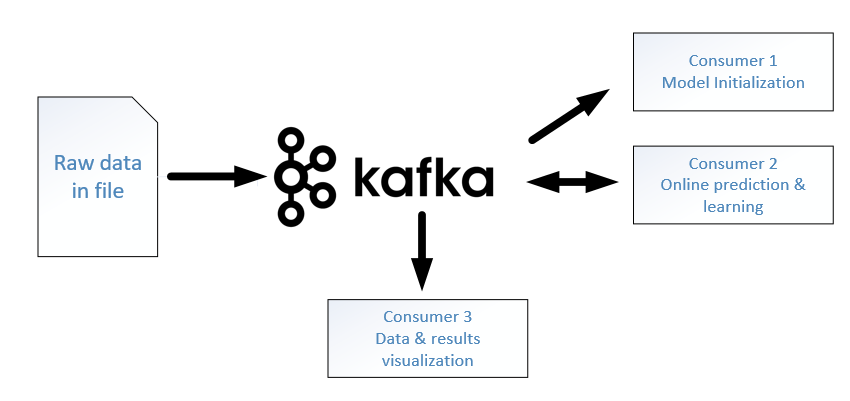
\includegraphics[width=10cm, height=5cm]{kafka}
\caption[Data stream Publisher-Consumer architecture]{Data stream Publisher-Consumer architecture}
\label{fig:kafka}
\end{figure}

For each dataset, we use around 20\% data for initialization and the other half for online prediction. Each subset used for training and prediction are preprocessed locally in batch, in order to scale them into $[0,1]$ to fit the LSTM activation function.


\section{Parameter tuning}
\label{sec:parametertuning}

For each dataset, we carry out a grid search step to tune the model hyperparameters. Here we try multiple combinations of window length and hidden size for each data set. The grid search set GS contains 5\% -15\% anomalies. Because of the uncertainty of the random neural network weight initialization, we do each experiment 10 times and take the average result to reduce the impact. To be noted that during every divisions, the consistency of streaming data is persisted, or in other words, there is no random sampling during the process. A good model should make the reconstruction error as large as possible in order to make the classification easier. Given dataset D,  'win' is the input window, the average reconstruction error of D is given by \Fref{eq:are}. The target function of grid search is given by the ration of average reconstruction error of abnormal and normal test grid search set GS (\Fref{eq:are}).

\begin{equation}\label{eq:are}
ARE(D) = \frac{1}{T}\sum_{t=1,win\in D}^{T}(input_{t,win}-output_{t,win})
\end{equation}

\begin{equation}\label{eq:ratio}
REratio=\frac{ARE(G_a)}{ARE(G_n)}
\end{equation}


As a result of grid search, the hyperparameters for different datasets are listed in Table~\ref{tab:hyper}.

\begin{table}[h] 
\caption{Hyperparameters} 
\centering      
\begin{tabular}{c c c c}  
\hline\hline        
Dataset & Window length & Hidden size & \#Grid Search instance \\ [0.5ex] 
\hline 
PowerDemand & 80 & 15 & 1 000 \\  
SMTP & 10 & 15 &  5 000 \\ 
SMTP+HTTP & 10 & 15 & 5 000 \\ 
HTTP & 30 & 35  &  10 000 \\ 
ForestCover & 10 & 25 & 10 000 \\ [1ex]  
\hline    
\end{tabular}
\label{tab:hyper}  
\end{table} 


\section{Streaming data generator: Apache Kafka}
\label{sec:Streaming data generator: Apache Kafka}

We utilize Apache Kafka as the streaming platform. Kafka is a widely used Publish/Subscribe architecture streaming system. It is different from classical message queue technique with its fault tolerant, durable and large capacity properties. Different application or database can publich data to a specific topic of Kafka (topic is the data category mechanisms used in Kafka), and other processors can consume data from this topic (\Fref{fig:kafkadiagram}). In our experimental setting, the data source is static databases, Kafka generate real-time data stream pipeline as data source publish records to the experiment topic, and furthermore the stream of records will be consumed by different consumers like our analysis model, visualization model etc. This configuration can be easily scaled up to more complicated and demanding real world use cases. Each record in the Kafka stream pipeline is in the form of [Key, Value, Timestamp], where keys are used for positioning and values carry the data record.

\begin{figure}[h]
\centering
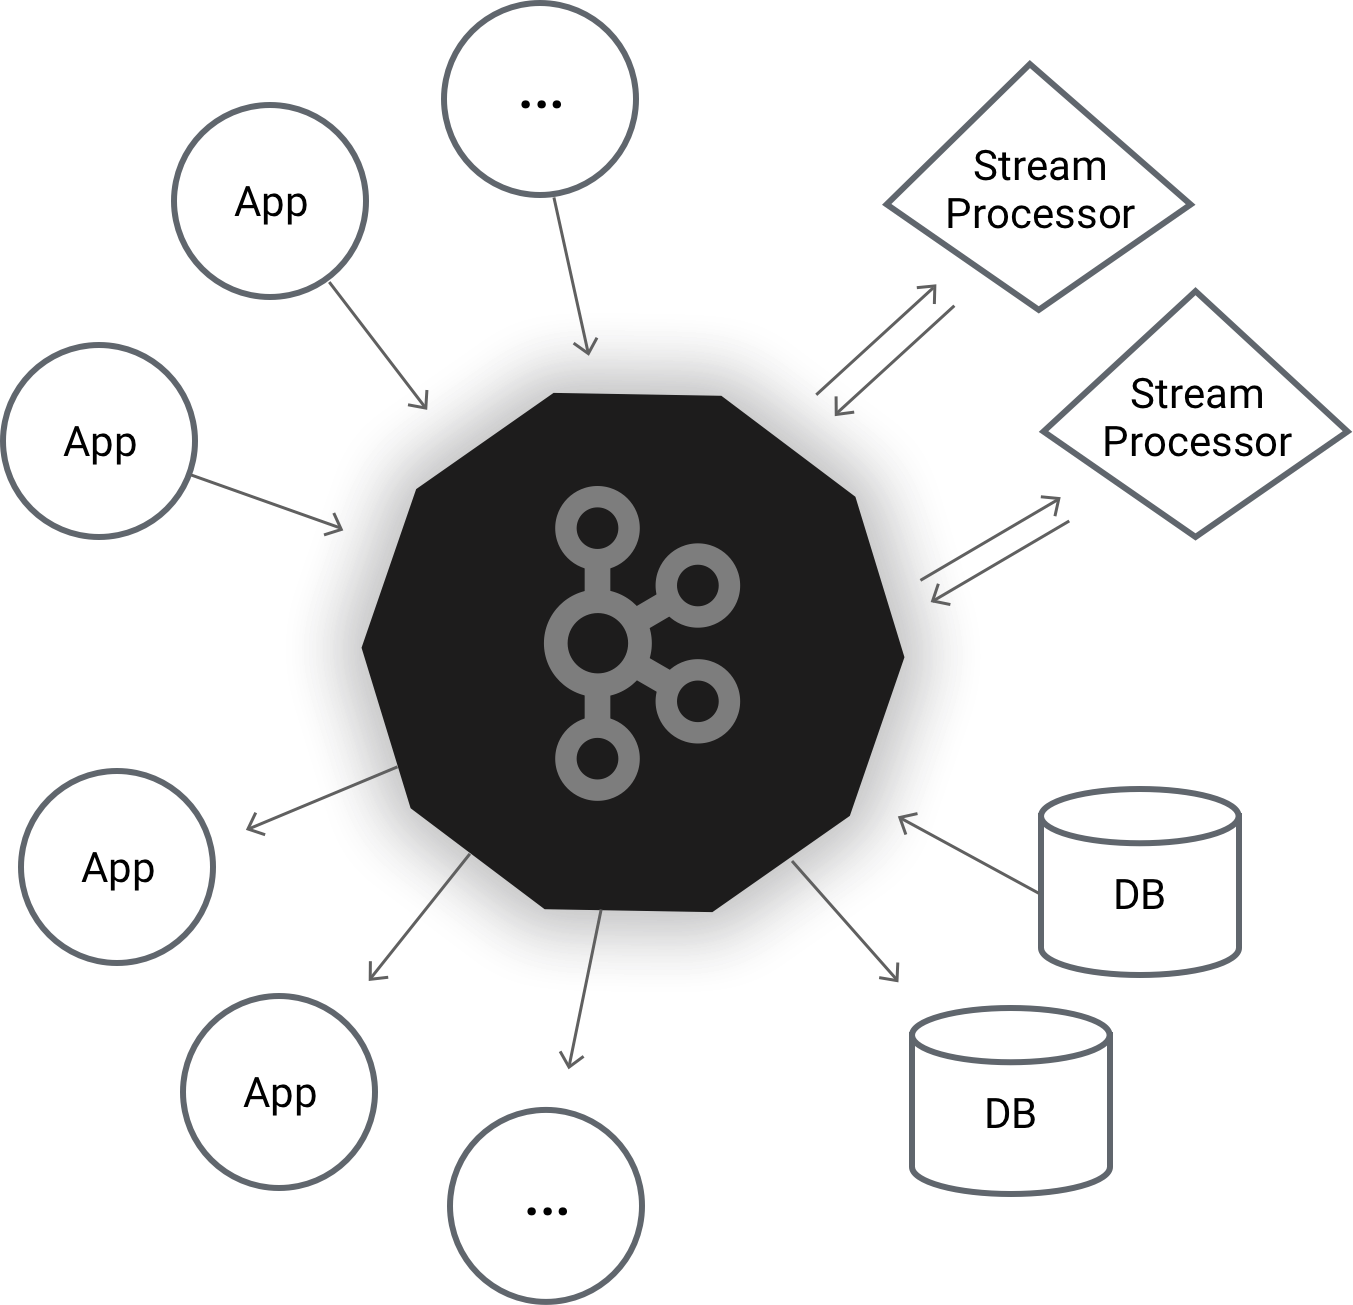
\includegraphics[width=5cm, height=5cm]{kafkadiagram}
\caption[Kafka diagram]{Kafka diagram\footnotemark}
\label{fig:kafkadiagram}
\end{figure}

\footnotetext{From: https://kafka.apache.org/}








